\documentclass[12pt]{article}
\usepackage{amsmath, amssymb, graphicx}
\usepackage[T1]{fontenc}
\usepackage[latin9]{inputenc}
\usepackage[margin=1in]{geometry} 
\usepackage{url}
\usepackage{amsthm,amsmath,amssymb}
\usepackage{mathrsfs}
\usepackage{makeidx}
\usepackage{microtype}
\usepackage{setspace}
\usepackage{graphicx}
\usepackage{ulem}
\usepackage{url}
\usepackage{enumerate}
\usepackage{tikz}
\usepackage{listings}
\usepackage{thmtools}
\usepackage{fancyhdr}
\usepackage{float}
\usepackage{tabularx}
\usepackage{ragged2e}
\usepackage{booktabs}
\usepackage{caption}
\usepackage{subcaption}
\usepackage{mathtools}
\usepackage{undertilde}
%\usepackage[nottoc]{tocbibind}

%\setlength{\textwidth}{6in}

\author{Amal Agarwal}
\title{Sparse Inverse Covariance Estimation using Graphical Lasso and BIGQUIC}
\date{\today}
\begin{document}
\maketitle

\section{Introduction} 
\label{sec:introduction}
The purpose of this survey is two-fold. At first, we explore the broad topic of graphical models which include two main subdivisions namely directed graph models or the so called "Beyesian networks" and undirected graphical models or "Markov graphical models". Secondly we go in deep to understand the methodology, advantages and implications behind the well known graphical Lasso procedure for estimating the structure and paramters of inverse covariance matrix in undirected gaussian graphical models. We will see how sparsity can be exploited in certain scenarios. In particular, we will focus on a state of the art algorithm BIGQUIC\cite{hsieh2013big} which can solve 1 million dimensional $l_1$ regularized Gaussian MLE problems using just 1 machine with 32 cores and 32G memory.

\section{Graphical models}
\label{gmodels}
A graph $G = (V,E)$ is formed by a collection of vertices
$V = \left\{1,2,...,p\right\}$, and a collection of edges $E\subset V\times V$. Each edge consists of a pair of vertices $s, t \in E$, and may either be undirected, in which case there is no distinction between edge $(s,t)$ and edge $(t,s)$, or directed, in which case we write $(s \rightarrow t)$ to indicate the direction.\cite{friedman2001elements}.

\subsection{Bayesian networks}
Bayesian networks are directed graphical models and belong to the family of probabilistic graphical models (PGMs). These are acyclic graphs with nodes representing random variables and the directed edges depicting the conditional independencies. These graphical structures are used to represent knowledge about an uncertain domain.\cite{ben2007bayesian}. Mathematically, a bayesian network can be represented by a joint distribution of the random variables $X_i, i=\left\{1,2,...,n\right\}$ via the chain rule as \[P(X_1,X_2,..., X_n)=\prod\limits_{i=1}^nP(X_i|Par_G(X_i))\]. Here $Par_G(X_i)$ depicts the parents of the node $X_i$ in the graph. One of the main advantages of using Bayesian networks is they facilitate modelling conditional indepencies which captures the essence of many real world distributions. In addition they can be useful to deal with missing data and hidden variables.

\begin{figure}[H]
  \centering
    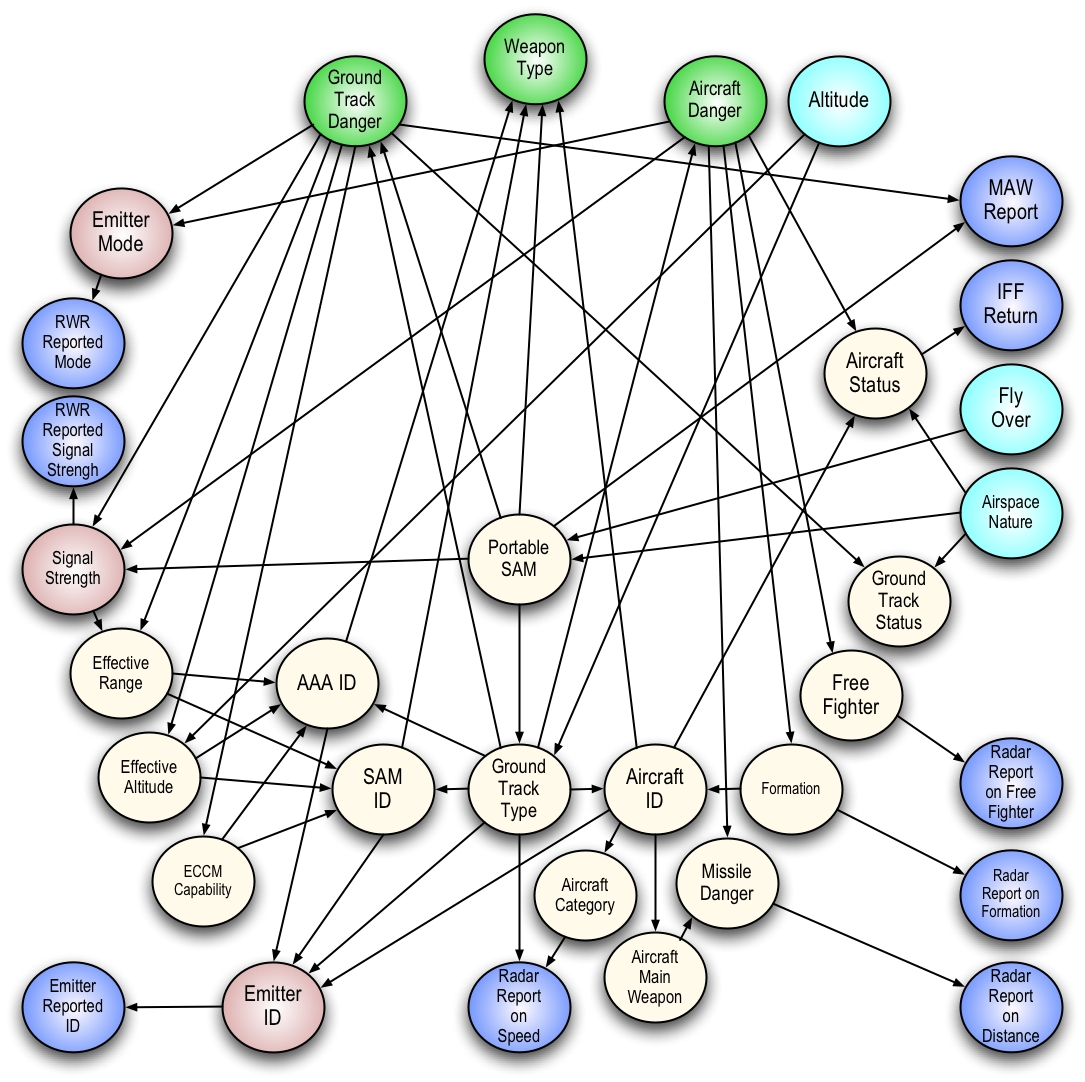
\includegraphics[width=0.50\textwidth]{fig1.jpg}
    \caption{An example of a Bayesian Network\cite{fig1}}
    \label{BN}
\end{figure}

\subsection{Markov random fields}
Markov random fields are undirected graphical models. Let us first define a few terms:
\begin{itemize}
\item \textbf{Subgraph}: A subgraph $U\in V$ is defined as the subset of vertices together with their edges.
\item \textbf{Clique}: A clique is a complete subgraph with a set of vertices that are all adjacent to one another.
\item \textbf{Maximal clique}: A clique is maximal if no other vertices can be added to it and still yield a clique.
\end{itemize}
Mathematically, markov random fields can be represented as a collection of ditributions that factorize as \[P(X_1,X_2,..., X_n)=\dfrac{1}{Z}\prod\limits_{C\in\mathcal{C}}\psi_C(x_C)\] Here $\mathcal{C}$ represents the set of maximal cliques and $\psi_C(.)$ are called clique potentials that capture the dependence of $X_c$ by scoring certain instances $x_C$ higher than others. Also $Z=\sum\limits_{x\in \mathcal{X}}\prod\limits_{C\in\mathcal{C}}\psi_C(x_C)$ is the normalizing constant and is called the partition function.

\begin{figure}[H]
  \centering
    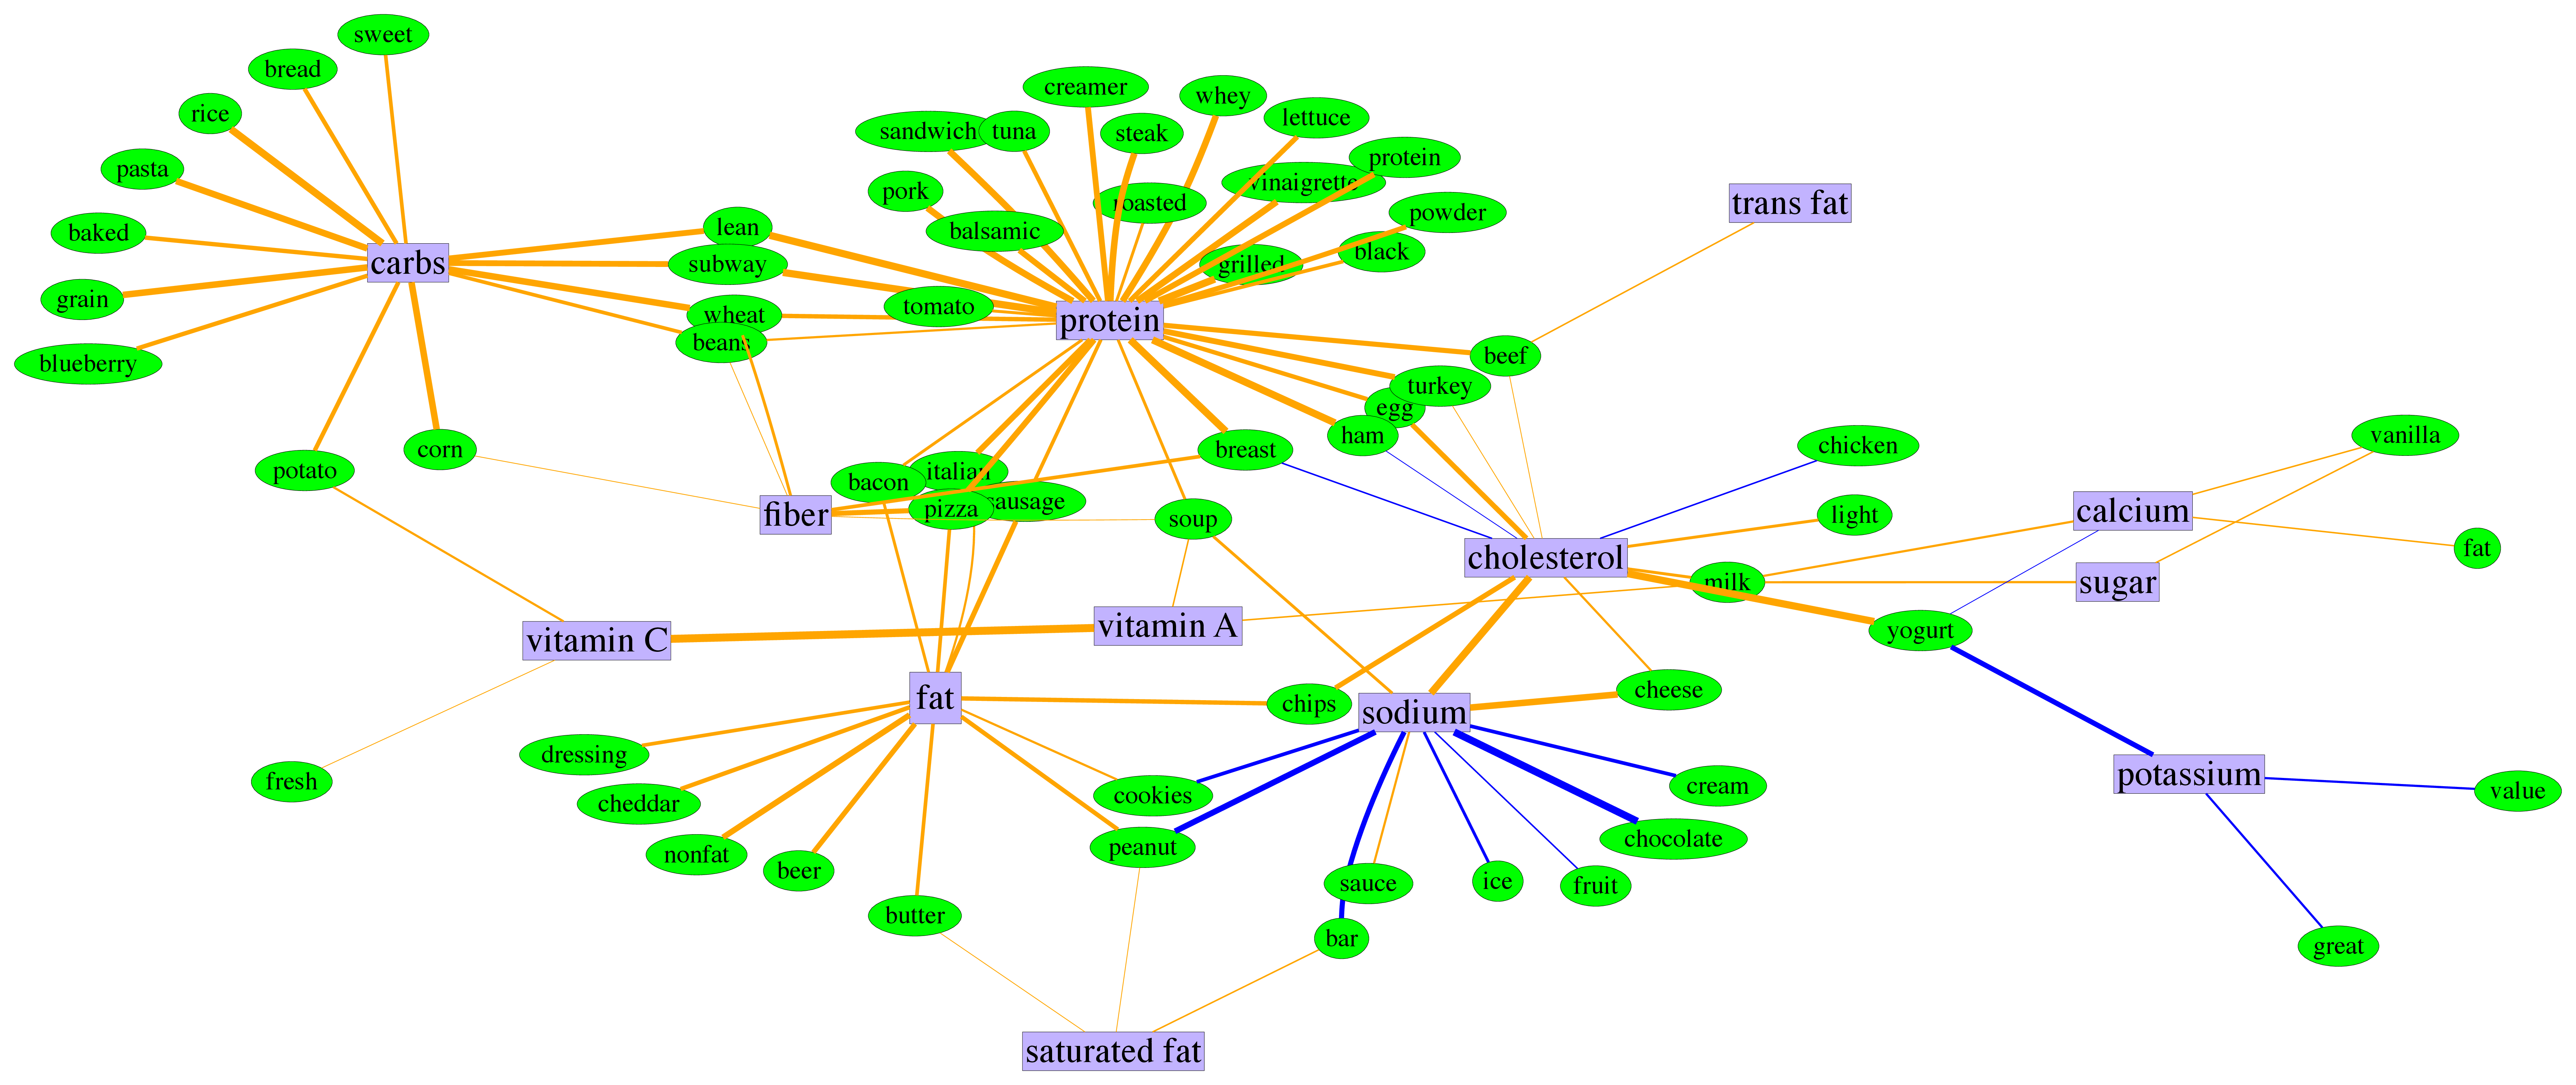
\includegraphics[width=0.75\textwidth]{fig2.png}
    \caption{An example of a Markov random field\cite{fig2}}
    \label{MRF}
\end{figure}

\section{Markov random fields for continuous variables}
When the node random variables follow continuous distributions, most of the time they are approximated by gaussian distribution due to their convenient analytical properties.\cite{friedman2001elements}. In this case, this is called as a Gaussian Random Markov Field (GMRF). For a GMRF with p nodes and n observations, we are generally interested in estimating the concentration matrix $C=\Sigma^{-1}$ where $\Sigma$ is the corresponding variance-covariance matrix. In particular this comprises of two steps:
\begin{itemize}
\item \textbf{Model Selection}: Identification of zero entries in the concentration matrix directly corresponds to finding the missing edges in the undirected graph. Missing edges imply conditional independencies. For example if there is no edge between the nodes $X^{(i)}$ and $X^{(j)}$, then there are independent given all the other random variables. This is the model selection in the Gaussian concentration graph model.
\item \textbf{Model estimation}: Once model selection is done, the structure of the graph gets fixed. Following this, estimation of the non-zero entries in the concentration matrix is done. Note that it is often convenient to use the concentration matrix since there are many stochastic processes (like AR1 time series) which guarantees sparseness of the matrix $C$ as opposed to working with $\Sigma$ directly. This sparseness can be exploited in different ways as we will discuss in later sections.
\end{itemize}

\subsection{Defining the problem}
We can write down the log-likelihood of the GMRF based on the random sample $\utilde{X_1},\utilde{X_2},..., \utilde{X_n}$ as\cite{yuan2007model}:\[l(\utilde{\mu},C)=\dfrac{n}{2}log|C|-\dfrac{1}{2}\sum\limits_{i=1}^{n}(\utilde{X_i}-\utilde{\mu})^T(\utilde{X_i}-\utilde{\mu})\]
The maximum likelihood estimator of $(\utilde{\mu},\Sigma)$ is $(\overline{X},\overline{A})$, where \[\overline{A}=\dfrac{1}{n}\sum\limits_{i=1}^n(\utilde{X_i}-\utilde{\overline{X}})^T(\utilde{X_i}-\utilde{\overline{X}})\]

The concentration matrix can then be estimated by $\hat{C}=\overline{A}^{-1}$ or $\hat{C}=S^{-1}$ where S is the sample covariance matrix defined as $S=\overline{A}^{-1}$ However for a large $p$, the number of parameters to be estimated is even larger $\dfrac{p(p+1)}{2}$. This leads to an unstablility of $\hat{C}$, that is small perturbations in the data leads to large fluctuations in elements of $\hat{C}$. Also, in general, this does not lead to sparseness in the corresponding graph since the matrix typically contains no zero entry.\cite{yuan2007model}

To resolve this problem, a common approach is introduce a $l_1$ Lasso penalty term in the log likelihood function by putting the following constraint. \[\sum\limits_{i\neq j}|c_{ij}|\leq t\]

Clearly $\hat{\mu}=\overline{X}$ and since the observations can be assumed to be centered without any loss of generality we can put $\hat{\mu}=0$. This leads us to the problem of minimizing the following negative log likelihood function
\begin{equation}
l(C)=-\text{log}|C|+\dfrac{1}{n}\sum\limits_{i=1}^n\utilde{X_i}^TC\utilde{X_i} \hspace{0.5in}\text{subject to}\hspace{0.5in} \sum\limits_{i\neq j}|c_{ij}|\leq t
\end{equation}
Note that 
\begin{equation*}
\begin{aligned}
\dfrac{1}{n}\sum\limits_{i=1}^n\utilde{X_i}^TC\utilde{X_i}&=\dfrac{1}{n}\sum\limits_{i=1}^ntr(\utilde{X_i}^TC\utilde{X_i})\\&=\dfrac{1}{n}\sum\limits_{i=1}^ntr(C\utilde{X_i}\utilde{X_i}^T)\\&=tr\left(C\left[\dfrac{1}{n}\sum\limits_{i=1}^n\utilde{X_i}\utilde{X_i}^T\right]\right)\\&=tr(C\overline{A})
\end{aligned}
\end{equation*}
Thus (1) becomes \[l(C)=-\text{log}|C|+tr(C\overline{A}) \hspace{0.5in}\text{subject to}\hspace{0.5in} \sum\limits_{i\neq j}|c_{ij}|\leq t\] Since both the objective function and the feasible region are convex, we can equivalently use the Lagrangian form \[-\text{log}|C|+tr(C\overline{A})+\lambda\sum\limits_{i\neq j}|c_{ij}|\]
where $\lambda$ is the tuning parameter.

This can also be rephrased as minimizing the function 
\begin{equation}
-\text{log}|C|+tr(C\overline{A})+\lambda||C||_1
\end{equation}

This is a convex optimization problem and is very difficult to solve mainly because of the non-smooth norm 1 term coupled with the smooth log determinant program. Various techniques have been proposed in the literature to deal with this problem. Here will focus primarily on Graphical Lasso and BIGQUIC algorithms.


\section{Graphical Lasso}
Let $W$ be the estimate of $\Sigma$. We can solve the problem by optimizing over each row and corresponding column of W in a block coordinate descent fashion.\cite{banerjee2008model}\cite{friedman2008sparse} Partitioning $W$ and $S$ as \[\begin{bmatrix}W_{11}& w_{12} \\w_{12}^T & w_{22}\end{bmatrix}\hspace{0.5in}\begin{bmatrix}S_{11}& s_{12} \\s_{12}^T & s_{22}\end{bmatrix}\] It can be shown that the solution for $w_{12}$ satisfies
\begin{equation}
w_{12} = \text{argmin}_y\left\{ y^TW_{11}^{-1}y : ||y-s_{12}||_{\infty} \leq \rho\right\}
\end{equation}
Using covex duality, it can be shown that (3) can be solved by solving the corresponding dual problem as 
\begin{equation}
\text{min}_\beta\left\{\dfrac{1}{2}||W_{11}^{1/2}\beta-b||^2+\rho||\beta||_1\right\}
\end{equation}
where $b=W_{11}^{-1/2}s_{12}$. If $\beta$ solves (4), then $w_{12}=W_{11}\beta$ is the solution of (3). 
The following Graphical Lasso algorithm\cite{friedman2008sparse} can be used to solve the optimization problem given in (3.1):
\begin{itemize}
\item Start with $W = S +\rho I$. The diagonal of $W$ remains unchanged
in what follows.
\item For each $j = 1, 2, . . . p$, solve the lasso problem (3), which takes as input the inner products $W_{11}$ and $s_{12}$. This gives a $p-1$ vector solution $\hat{\beta}$. Fill in the corresponding row and column of $W$ using $w_{12} = W_{11}\hat{\beta}$.
\item Continue until convergence.
\end{itemize}
This is a simple and fast algorithm for estimation of a sparse inverse covariance matrix using an $L_1$ penalty. It cycles through the variables, fitting a modified lasso regression to each variable in turn. The individual lasso problems are solved by coordinate descent. The speed of this new procedure can facilitate the application of sparse inverse covariance procedures to large datasets involving thousands of parameters.\cite{friedman2008sparse}

\section{BIGQUIC}
The above Graphical Lasso algorithm along with many state of the art techniques do not scale to problems for more than $20,000$ variables. The BIGQUIC algorithm\cite{hsieh2013big} can solve 1 million dimensional $l_1$ regularized Gaussian MLE problems (with 1000 billion parameters) using a single machine with bounded memory. BIGQUIC is based on QUIC and therefore we will first review QUIC briefly.
\subsection{Review of QUIC} 
QUIC is the state of the art procedure for solving (2) based on a second order optimization method. We will review this algorithm and explore the key bottlenecks that arise when scaling it to a million parameters\cite{hsieh2013big}.
QUIC iteratively solves for the generalized Newton direction using coordinate descent and then descends using this Newton direction and line search. Since the objective function of (2) is non-smooth we can separate the smooth and non-smooth part by $f(C)=g(C)+h(C)$ where $g(C)=-\text{log}|C|+tr(SC)$ and $h(C)=\lambda||C||_1$. To exploit the sparsity of the solution, the variables are partitioned into $S_{\text{fixed}}$ and $S_{\text{free}}$ sets: i.e. $C_{ij}\in S_{\text{fixed}}$ if $|\nabla_{ij}g(C)|\leq\lambda_{ij}$ and $C_{ij}=0$. Otherwise $C_{ij}\in S_{\text{free}}$. Only the free set $S_{\text{free}}$is updated at each Newton iteration, reducing the number of variables to be updated to $m=|S_{\text{free}}|$, which is comparable to $||C*||_0$, the sparsity of the solution.
The generalized Newton direction for (2) is \[D_t=\text{argmin}_D\left\{\overline{g}_{C_t}(D)+h(C_t+D)\right\}\]
where \[\overline{g}_{C_t}(D)=g(C_t)+tr(\nabla g(C_t)^TD)+\dfrac{1}{2}\text{vec}(D)^T\nabla^2g(C_t)\text{vec}(D)\]
In this problem it can be shown that $\nabla g(C_t)=S-C_{t}^{-1}$ and $\nabla^2g(C)=C_{t}^{-1}\otimes C_{t}^{-1}$. When $C_t$ is sparse, the Newton direction computation can be solved efficiently by the coordinate decent. This can be implemented by computing and storing $W_t=C_t^{-1}$, uding tihis to compute $a=W_{ij}^2+W_{ii}W_{jj}$, $b=S_{ij}-W_{ij}+w_i^TDw_j$ and $c=C_{ij}+D_{ij}$. With this quantities, the coordinate descent update for variable $D_{ij}$ takes the form $D_{ij}\leftarrow D_{ij}-c+\mathcal{S}(c-b/a,\lambda_{ij}/a)$ where $S(z,r)=sign(z)max(|z|-r,0)$ is the soft thresholding function.

\section{Bottlenecks of QUIC and their solutions}
\begin{itemize}
\item Terms of $w_i^TDw_j$ take $O(p^2)$. To resolve this problem, Block ccordinate descent methid can be used via clustering. This optimizes the memoy use and computational cost and exploits sparsity.
\item QUIC descends along the Newton's direction via Armijo's rule. This is done by first selecting the largest step $\alpha \in \{ \beta^{0},\beta^{1},...\}$ such that $C+\alpha D_t$ is positive definite and satisfies the constraint $f(C+\alpha D^{*}) \leq f(C)+\alpha\sigma\delta$ where $\delta=tr(\nabla g(C_t)^{T}D^{*})+||C+D^{*}||_{1}-||C||_1$. The bottlenecks here are to check the positive definiteness by computing the smallest eigenvalue using cholesky decomposition and to compute the determinant of a sparse matrix. The remedies suggested were use schur components instead and implememnt sparse linear equation solver.
\end{itemize}

\section{Extending QUIC to BIGQUIC}
The key steps of the BOIGQUIC are described here. First, Conjugate Gradient (CG) method can be used to compute $\utilde{w_i}$ by solving the system $C\utilde{w_i}=\utilde{e_i}$, using the fact that X is a positive definite matrix. This step has time complexity $O(mT)$ where $m$ is the number  non-zero elements in $C_t$ and T is the number of iterations required to achieve the desired accuracy. For the update step of $D_{ij}$ in QUIC, booth $\utilde{w_i}$ and $\utilde{w_j}$ are needed. If either one is not available, CG has to be used to recompute it and this is callled as a "cache miss". The goal here is to minimize this cache miss rate. The following block by block clustering method via clustering scheme was applied to mimimize this cache miss rate.

\subsection{Block coordinate descent}
Number of blocks were chosen as $k$ so that $\dfrac{p}{k}$ columns of $W$ can be stored in memory. The blocks were represented as $S_1, S_2,..., S_k $. $D$ was then divided into $k\times k$ blocks accordingly. $T_{\text{inner}}$ is the number of iterations over variables within a particular block and $T_{\text{outer}}$ is the number of iterations through all the blocks. Let $W_{S_q}$ denotes the $p\times |S_q|$ matrix containing columns of $W$ that corresponds to the subset $S_q$.

\subsection{Coordinate descent within a block}
To update the variables in the block $S_z, S_q$, of $D$, first $W_{S_z}$ and $W_{S_q}$ are computed by CG and stored in the memory so that there is no cache miss during the within block coordinate updates. With $U_{S_q}=DW_{S_q}$ maintained,the update for $D_{ij}$ can be computed by $\utilde{w_i}^T\utilde{w_j}$, when $i \in S_z$ and $j \in S_q$. After updating each $D_{ij}$ to $D_{ij}+\mu$, $U_{S_q}$ is maintained as \[U_{it}\leftarrow U_{it}+\mu W_{jt}, \hspace{0.2in} U_{jt}\leftarrow U_{jt}+\mu W_{it} \forall t \in S_q\]
The above coordinate update computations costs only $O(p/k)$ since this involves only a subset of columns. Note that $U_{rt}$ never changes when $r \not\in {S_z \cup S_q}$. 
Before running coordinate descent for the block, $P_{ij}=(w_{i})_{S_{\overline{z}\overline{q}}}^{T}(u_j)_{S_{\overline{z}\overline{q}}}$ are computed $\forall(i,j)$ in the free set of the current block. Here  $S_{\overline{z}\overline{q}}=\left\{i|i\not\in S_z \text{and} i\not\in S_q\right\}$. The term $\utilde{w_i}^T\utilde{u_j}$ for updating $D_{ij}$ can then be computed by $w_{i}^{T}u_{j}=P_{ij}+w_{S_{z}}^{T}u_{S_{z}}+w_{S_{q}}^{T}u_{S_{q}}$. With this trick each coordinate descent step takes only $O(p/k)$ time and we need to store only $U_{S_z, S_q}$ which requires $O(p^2/k^2)$ memory.

\subsection{Sweeping through all the blocks}
To go through all the blocks, each time a $z\in \left\{1,..., k\right\}$ is selected and blocks $(S_z,S_1),..., (S_z,S_k)$ are updated. Since all them share $\utilde{w_i}|i\in S_z$, these are first computed and stored in the memory. When updating an off-diagonal block $(S_z,S_q)$, if the free sets are dense,  $\utilde{w_i}|i\in S_z$ is computed and stored first. So totally each block of $W$ is computed $k$ times and the total time complexity becomes $O(kpmt)$.

 \subsection{Selecting the blocks through clustering}
 While updating the block $(S_z, S_q)$, $w_j$ is required only if some variable in $\{D_{ij}|i \in S_z\}$ lies in the free set. Boundary nodes are defined as $B(S_z, S_q)=\{j|j\in S_q \text{ and } \exists i \in S_z$ s.t. $F_{ij}=1\}$ where F is indicator of free set. The number of columns computed in one sweep is  $p+\displaystyle\sum_{z\neq q}|B(S_z, S_q)|$. However, the boundary nodes bounded by cross cluster edges are  $B(S_z, S_q)<\sum_{i \in S_z, j\in S_q}F_{ij}$. Graph clustering algorithms like METIS minimizes RHS. The time complexity is reduced to  $O((p+rm)T)$
 
 \subsection{Line search}
The following procedure was adopted as a n effocient and scalable procedure to compute $\text{log}|A|$,\[log det(A)=\displaystyle\sum_{i=1}^{p}log(A_{ii}-A_{(i+1):p,i}^{T}A_{(i+1):p,(i+1):p}^{-1}A_{(i+1):p,i}) \]

\section{Discussion}
In this survey, we briefly went over Graphical Lasso and BIGQUIC algorithms to solve the inverse covariance estimation problem. We saw that while Graphical Lasso is simple and easy to implement, BIGQUIC can scale upto 1 million variable problems. This has a lot of applications in extremely high dimensional datasets.

\bibliography{bibfile}{}
\bibliographystyle{ieeetr} 
\end{document}
